\documentclass[1p]{elsarticle_modified}
%\bibliographystyle{elsarticle-num}

%\usepackage[colorlinks]{hyperref}
%\usepackage{abbrmath_seonhwa} %\Abb, \Ascr, \Acal ,\Abf, \Afrak
\usepackage{amsfonts}
\usepackage{amssymb}
\usepackage{amsmath}
\usepackage{amsthm}
\usepackage{scalefnt}
\usepackage{amsbsy}
\usepackage{kotex}
\usepackage{caption}
\usepackage{subfig}
\usepackage{color}
\usepackage{graphicx}
\usepackage{xcolor} %% white, black, red, green, blue, cyan, magenta, yellow
\usepackage{float}
\usepackage{setspace}
\usepackage{hyperref}

\usepackage{tikz}
\usetikzlibrary{arrows}

\usepackage{multirow}
\usepackage{array} % fixed length table
\usepackage{hhline}

%%%%%%%%%%%%%%%%%%%%%
\makeatletter
\renewcommand*\env@matrix[1][\arraystretch]{%
	\edef\arraystretch{#1}%
	\hskip -\arraycolsep
	\let\@ifnextchar\new@ifnextchar
	\array{*\c@MaxMatrixCols c}}
\makeatother %https://tex.stackexchange.com/questions/14071/how-can-i-increase-the-line-spacing-in-a-matrix
%%%%%%%%%%%%%%%

\usepackage[normalem]{ulem}

\newcommand{\msout}[1]{\ifmmode\text{\sout{\ensuremath{#1}}}\else\sout{#1}\fi}
%SOURCE: \msout is \stkout macro in https://tex.stackexchange.com/questions/20609/strikeout-in-math-mode

\newcommand{\cancel}[1]{
	\ifmmode
	{\color{red}\msout{#1}}
	\else
	{\color{red}\sout{#1}}
	\fi
}

\newcommand{\add}[1]{
	{\color{blue}\uwave{#1}}
}

\newcommand{\replace}[2]{
	\ifmmode
	{\color{red}\msout{#1}}{\color{blue}\uwave{#2}}
	\else
	{\color{red}\sout{#1}}{\color{blue}\uwave{#2}}
	\fi
}

\newcommand{\Sol}{\mathcal{S}} %segment
\newcommand{\D}{D} %diagram
\newcommand{\A}{\mathcal{A}} %arc


%%%%%%%%%%%%%%%%%%%%%%%%%%%%%5 test

\def\sl{\operatorname{\textup{SL}}(2,\Cbb)}
\def\psl{\operatorname{\textup{PSL}}(2,\Cbb)}
\def\quan{\mkern 1mu \triangleright \mkern 1mu}

\theoremstyle{definition}
\newtheorem{thm}{Theorem}[section]
\newtheorem{prop}[thm]{Proposition}
\newtheorem{lem}[thm]{Lemma}
\newtheorem{ques}[thm]{Question}
\newtheorem{cor}[thm]{Corollary}
\newtheorem{defn}[thm]{Definition}
\newtheorem{exam}[thm]{Example}
\newtheorem{rmk}[thm]{Remark}
\newtheorem{alg}[thm]{Algorithm}

\newcommand{\I}{\sqrt{-1}}
\begin{document}

%\begin{frontmatter}
%
%\title{Boundary parabolic representations of knots up to 8 crossings}
%
%%% Group authors per affiliation:
%\author{Yunhi Cho} 
%\address{Department of Mathematics, University of Seoul, Seoul, Korea}
%\ead{yhcho@uos.ac.kr}
%
%
%\author{Seonhwa Kim} %\fnref{s_kim}}
%\address{Center for Geometry and Physics, Institute for Basic Science, Pohang, 37673, Korea}
%\ead{ryeona17@ibs.re.kr}
%
%\author{Hyuk Kim}
%\address{Department of Mathematical Sciences, Seoul National University, Seoul 08826, Korea}
%\ead{hyukkim@snu.ac.kr}
%
%\author{Seokbeom Yoon}
%\address{Department of Mathematical Sciences, Seoul National University, Seoul, 08826,  Korea}
%\ead{sbyoon15@snu.ac.kr}
%
%\begin{abstract}
%We find all boundary parabolic representation of knots up to 8 crossings.
%
%\end{abstract}
%\begin{keyword}
%    \MSC[2010] 57M25 
%\end{keyword}
%
%\end{frontmatter}

%\linenumbers
%\tableofcontents
%
\newcommand\colored[1]{\textcolor{white}{\rule[-0.35ex]{0.8em}{1.4ex}}\kern-0.8em\color{red} #1}%
%\newcommand\colored[1]{\textcolor{white}{ #1}\kern-2.17ex	\textcolor{white}{ #1}\kern-1.81ex	\textcolor{white}{ #1}\kern-2.15ex\color{red}#1	}

{\Large $\underline{11n_{155}~(K11n_{155})}$}

\setlength{\tabcolsep}{10pt}
\renewcommand{\arraystretch}{1.6}
\vspace{1cm}\begin{tabular}{m{100pt}>{\centering\arraybackslash}m{274pt}}
\multirow{5}{120pt}{
	\centering
	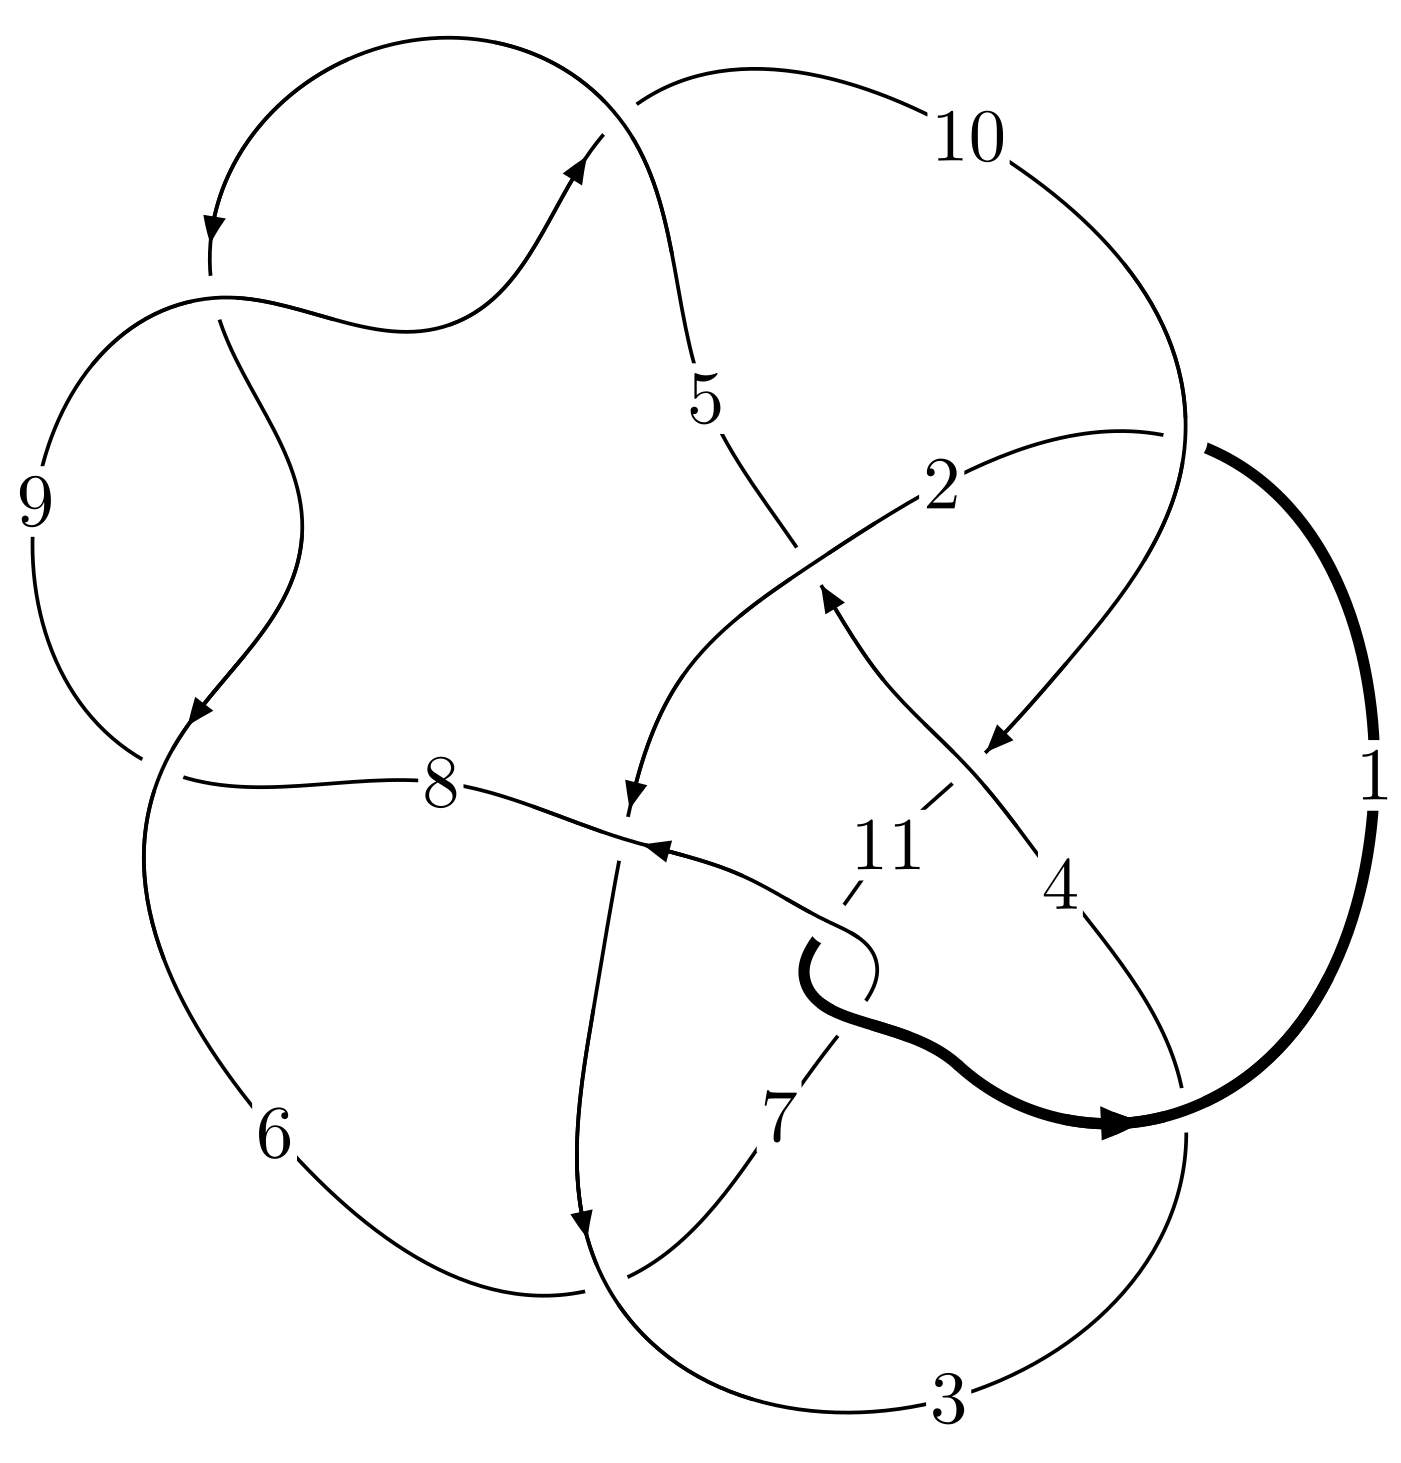
\includegraphics[width=112pt]{../../../GIT/diagram.site/Diagrams/png/771_11n_155.png}\\
\ \ \ A knot diagram\footnotemark}&
\allowdisplaybreaks
\textbf{Linearized knot diagam} \\
\cline{2-2}
 &
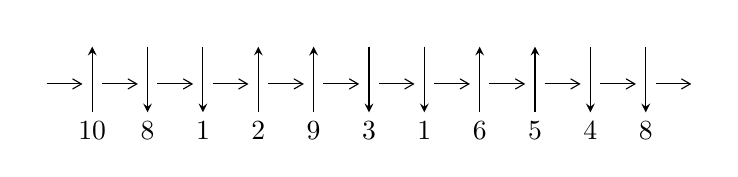
\begin{tikzpicture}[x=20pt, y=17pt]
	% nodes
	\node (C0) at (0, 0) {};
	\node (C1) at (1, 0) {};
	\node (C1U) at (1, +1) {};
	\node (C1D) at (1, -1) {10};

	\node (C2) at (2, 0) {};
	\node (C2U) at (2, +1) {};
	\node (C2D) at (2, -1) {8};

	\node (C3) at (3, 0) {};
	\node (C3U) at (3, +1) {};
	\node (C3D) at (3, -1) {1};

	\node (C4) at (4, 0) {};
	\node (C4U) at (4, +1) {};
	\node (C4D) at (4, -1) {2};

	\node (C5) at (5, 0) {};
	\node (C5U) at (5, +1) {};
	\node (C5D) at (5, -1) {9};

	\node (C6) at (6, 0) {};
	\node (C6U) at (6, +1) {};
	\node (C6D) at (6, -1) {3};

	\node (C7) at (7, 0) {};
	\node (C7U) at (7, +1) {};
	\node (C7D) at (7, -1) {1};

	\node (C8) at (8, 0) {};
	\node (C8U) at (8, +1) {};
	\node (C8D) at (8, -1) {6};

	\node (C9) at (9, 0) {};
	\node (C9U) at (9, +1) {};
	\node (C9D) at (9, -1) {5};

	\node (C10) at (10, 0) {};
	\node (C10U) at (10, +1) {};
	\node (C10D) at (10, -1) {4};

	\node (C11) at (11, 0) {};
	\node (C11U) at (11, +1) {};
	\node (C11D) at (11, -1) {8};
	\node (C12) at (12, 0) {};

	% arrows
	\draw[->,>={angle 60}]
	(C0) edge (C1) (C1) edge (C2) (C2) edge (C3) (C3) edge (C4) (C4) edge (C5) (C5) edge (C6) (C6) edge (C7) (C7) edge (C8) (C8) edge (C9) (C9) edge (C10) (C10) edge (C11) (C11) edge (C12) ;	\draw[->,>=stealth]
	(C1D) edge (C1U) (C2U) edge (C2D) (C3U) edge (C3D) (C4D) edge (C4U) (C5D) edge (C5U) (C6U) edge (C6D) (C7U) edge (C7D) (C8D) edge (C8U) (C9D) edge (C9U) (C10U) edge (C10D) (C11U) edge (C11D) ;
	\end{tikzpicture} \\
\hhline{~~} \\& 
\textbf{Solving Sequence} \\ \cline{2-2} 
 &
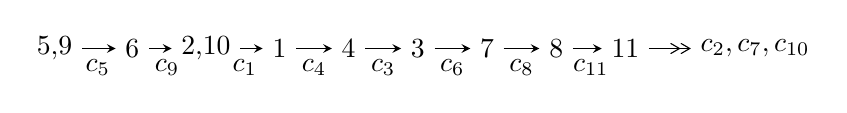
\begin{tikzpicture}[x=25pt, y=7pt]
	% node
	\node (A0) at (-1/8, 0) {5,9};
	\node (A1) at (1, 0) {6};
	\node (A2) at (33/16, 0) {2,10};
	\node (A3) at (25/8, 0) {1};
	\node (A4) at (33/8, 0) {4};
	\node (A5) at (41/8, 0) {3};
	\node (A6) at (49/8, 0) {7};
	\node (A7) at (57/8, 0) {8};
	\node (A8) at (65/8, 0) {11};
	\node (C1) at (1/2, -1) {$c_{5}$};
	\node (C2) at (3/2, -1) {$c_{9}$};
	\node (C3) at (21/8, -1) {$c_{1}$};
	\node (C4) at (29/8, -1) {$c_{4}$};
	\node (C5) at (37/8, -1) {$c_{3}$};
	\node (C6) at (45/8, -1) {$c_{6}$};
	\node (C7) at (53/8, -1) {$c_{8}$};
	\node (C8) at (61/8, -1) {$c_{11}$};
	\node (A9) at (10, 0) {$c_{2},c_{7},c_{10}$};

	% edge
	\draw[->,>=stealth]	
	(A0) edge (A1) (A1) edge (A2) (A2) edge (A3) (A3) edge (A4) (A4) edge (A5) (A5) edge (A6) (A6) edge (A7) (A7) edge (A8) ;
	\draw[->>,>={angle 60}]	
	(A8) edge (A9);
\end{tikzpicture} \\ 

\end{tabular} \\

\footnotetext{
The image of knot diagram is generated by the software ``\textbf{Draw programme}" developed by Andrew Bartholomew(\url{http://www.layer8.co.uk/maths/draw/index.htm\#Running-draw}), where we modified some parts for our purpose(\url{https://github.com/CATsTAILs/LinksPainter}).
}\phantom \\ \newline 
\centering \textbf{Ideals for irreducible components\footnotemark of $X_{\text{par}}$} 
 
\begin{align*}
I^u_{1}&=\langle 
u^{17}+5 u^{16}+\cdots+b+1,\;u^{17}+7 u^{16}+\cdots+2 a+17,\;u^{18}+5 u^{17}+\cdots+13 u+2\rangle \\
I^u_{2}&=\langle 
u^5+u^4+3 u^3+2 u^2+b+2 u,\;u^5+2 u^4+4 u^3+5 u^2+a+4 u+2,\\
\phantom{I^u_{2}}&\phantom{= \langle  }u^9+2 u^8+7 u^7+10 u^6+16 u^5+15 u^4+12 u^3+5 u^2-1\rangle \\
I^u_{3}&=\langle 
u^7 a+4 u^7+5 u^5 a-7 u^6+u^4 a+20 u^5+8 u^3 a-24 u^4+4 u^2 a+25 u^3+6 a u-19 u^2+7 b- a+3 u+3,\\
\phantom{I^u_{3}}&\phantom{= \langle  }u^6 a+u^7-2 u^5 a+5 u^4 a+4 u^5-6 u^3 a- u^4+6 u^2 a+5 u^3+a^2-4 a u-3 u^2+a+u+2,\\
\phantom{I^u_{3}}&\phantom{= \langle  }u^8- u^7+5 u^6-4 u^5+7 u^4-4 u^3+2 u^2+1\rangle \\
\\
\end{align*}
\raggedright * 3 irreducible components of $\dim_{\mathbb{C}}=0$, with total 43 representations.\\
\footnotetext{All coefficients of polynomials are rational numbers. But the coefficients are sometimes approximated in decimal forms when there is not enough margin.}
\newpage
\renewcommand{\arraystretch}{1}
\centering \section*{I. $I^u_{1}= \langle u^{17}+5 u^{16}+\cdots+b+1,\;u^{17}+7 u^{16}+\cdots+2 a+17,\;u^{18}+5 u^{17}+\cdots+13 u+2 \rangle$}
\flushleft \textbf{(i) Arc colorings}\\
\begin{tabular}{m{7pt} m{180pt} m{7pt} m{180pt} }
\flushright $a_{5}=$&$\begin{pmatrix}1\\0\end{pmatrix}$ \\
\flushright $a_{9}=$&$\begin{pmatrix}0\\u\end{pmatrix}$ \\
\flushright $a_{6}=$&$\begin{pmatrix}1\\- u^2\end{pmatrix}$ \\
\flushright $a_{2}=$&$\begin{pmatrix}-\frac{1}{2} u^{17}-\frac{7}{2} u^{16}+\cdots-42 u-\frac{17}{2}\\- u^{17}-5 u^{16}+\cdots-14 u-1\end{pmatrix}$ \\
\flushright $a_{10}=$&$\begin{pmatrix}u\\u\end{pmatrix}$ \\
\flushright $a_{1}=$&$\begin{pmatrix}-\frac{1}{2} u^{17}-\frac{7}{2} u^{16}+\cdots-30 u-\frac{13}{2}\\- u^{17}-5 u^{16}+\cdots-2 u+1\end{pmatrix}$ \\
\flushright $a_{4}=$&$\begin{pmatrix}\frac{1}{2} u^{17}+\frac{3}{2} u^{16}+\cdots-10 u-\frac{5}{2}\\- u^{17}-5 u^{16}+\cdots-20 u-3\end{pmatrix}$ \\
\flushright $a_{3}=$&$\begin{pmatrix}-\frac{3}{2} u^{17}-\frac{15}{2} u^{16}+\cdots-45 u-\frac{17}{2}\\- u^{17}-4 u^{16}+\cdots-2 u^2+1\end{pmatrix}$ \\
\flushright $a_{7}=$&$\begin{pmatrix}-\frac{1}{2} u^{17}-\frac{5}{2} u^{16}+\cdots-6 u-\frac{1}{2}\\- u^{16}-4 u^{15}+\cdots-6 u-1\end{pmatrix}$ \\
\flushright $a_{8}=$&$\begin{pmatrix}- u\\u^3+u\end{pmatrix}$ \\
\flushright $a_{11}=$&$\begin{pmatrix}-\frac{1}{2} u^{17}-\frac{7}{2} u^{16}+\cdots-29 u-\frac{13}{2}\\- u^{17}-5 u^{16}+\cdots-3 u+1\end{pmatrix}$\\ \flushright $a_{11}=$&$\begin{pmatrix}-\frac{1}{2} u^{17}-\frac{7}{2} u^{16}+\cdots-29 u-\frac{13}{2}\\- u^{17}-5 u^{16}+\cdots-3 u+1\end{pmatrix}$\\&\end{tabular}
\flushleft \textbf{(ii) Obstruction class $= -1$}\\~\\
\flushleft \textbf{(iii) Cusp Shapes $= 4 u^{17}+19 u^{16}+83 u^{15}+236 u^{14}+583 u^{13}+1152 u^{12}+1976 u^{11}+2870 u^{10}+3638 u^9+3961 u^8+3775 u^7+3072 u^6+2159 u^5+1248 u^4+580 u^3+175 u^2+39 u-4$}\\~\\
\newpage\renewcommand{\arraystretch}{1}
\flushleft \textbf{(iv) u-Polynomials at the component}\newline \\
\begin{tabular}{m{50pt}|m{274pt}}
Crossings & \hspace{64pt}u-Polynomials at each crossing \\
\hline $$\begin{aligned}c_{1},c_{4}\end{aligned}$$&$\begin{aligned}
&u^{18}+u^{17}+\cdots-6 u+1
\end{aligned}$\\
\hline $$\begin{aligned}c_{2}\end{aligned}$$&$\begin{aligned}
&u^{18}-10 u^{16}+\cdots- u+23
\end{aligned}$\\
\hline $$\begin{aligned}c_{3}\end{aligned}$$&$\begin{aligned}
&u^{18}-11 u^{17}+\cdots-17 u+24
\end{aligned}$\\
\hline $$\begin{aligned}c_{5},c_{8},c_{9}\end{aligned}$$&$\begin{aligned}
&u^{18}+5 u^{17}+\cdots+13 u+2
\end{aligned}$\\
\hline $$\begin{aligned}c_{6},c_{7},c_{11}\end{aligned}$$&$\begin{aligned}
&u^{18}+u^{17}+\cdots+u+1
\end{aligned}$\\
\hline $$\begin{aligned}c_{10}\end{aligned}$$&$\begin{aligned}
&u^{18}+16 u^{17}+\cdots+1792 u+256
\end{aligned}$\\
\hline
\end{tabular}\\~\\
\newpage\renewcommand{\arraystretch}{1}
\flushleft \textbf{(v) Riley Polynomials at the component}\newline \\
\begin{tabular}{m{50pt}|m{274pt}}
Crossings & \hspace{64pt}Riley Polynomials at each crossing \\
\hline $$\begin{aligned}c_{1},c_{4}\end{aligned}$$&$\begin{aligned}
&y^{18}+11 y^{17}+\cdots-8 y+1
\end{aligned}$\\
\hline $$\begin{aligned}c_{2}\end{aligned}$$&$\begin{aligned}
&y^{18}-20 y^{17}+\cdots+597 y+529
\end{aligned}$\\
\hline $$\begin{aligned}c_{3}\end{aligned}$$&$\begin{aligned}
&y^{18}-23 y^{17}+\cdots-433 y+576
\end{aligned}$\\
\hline $$\begin{aligned}c_{5},c_{8},c_{9}\end{aligned}$$&$\begin{aligned}
&y^{18}+19 y^{17}+\cdots+47 y+4
\end{aligned}$\\
\hline $$\begin{aligned}c_{6},c_{7},c_{11}\end{aligned}$$&$\begin{aligned}
&y^{18}-27 y^{17}+\cdots-7 y+1
\end{aligned}$\\
\hline $$\begin{aligned}c_{10}\end{aligned}$$&$\begin{aligned}
&y^{18}+70 y^{16}+\cdots+262144 y+65536
\end{aligned}$\\
\hline
\end{tabular}\\~\\
\newpage\flushleft \textbf{(vi) Complex Volumes and Cusp Shapes}
$$\begin{array}{c|c|c}  
\text{Solutions to }I^u_{1}& \I (\text{vol} + \sqrt{-1}CS) & \text{Cusp shape}\\
 \hline 
\begin{aligned}
u &= -0.792060 + 0.657087 I \\
a &= \phantom{-}0.537685 + 0.783791 I \\
b &= -0.78194 + 1.18447 I\end{aligned}
 & -8.36952 - 8.49029 I & -4.40486 + 6.13776 I \\ \hline\begin{aligned}
u &= -0.792060 - 0.657087 I \\
a &= \phantom{-}0.537685 - 0.783791 I \\
b &= -0.78194 - 1.18447 I\end{aligned}
 & -8.36952 + 8.49029 I & -4.40486 - 6.13776 I \\ \hline\begin{aligned}
u &= \phantom{-}0.298470 + 0.918902 I \\
a &= \phantom{-}0.477719 - 0.191775 I \\
b &= \phantom{-}0.302221 + 0.080115 I\end{aligned}
 & -0.45845 + 1.47133 I & -0.00849 - 6.64687 I \\ \hline\begin{aligned}
u &= \phantom{-}0.298470 - 0.918902 I \\
a &= \phantom{-}0.477719 + 0.191775 I \\
b &= \phantom{-}0.302221 - 0.080115 I\end{aligned}
 & -0.45845 - 1.47133 I & -0.00849 + 6.64687 I \\ \hline\begin{aligned}
u &= -0.921919 + 0.489220 I \\
a &= -0.516597 + 0.056157 I \\
b &= -0.464186 - 0.991439 I\end{aligned}
 & -7.77265 + 2.85464 I & -5.54920 - 2.31741 I \\ \hline\begin{aligned}
u &= -0.921919 - 0.489220 I \\
a &= -0.516597 - 0.056157 I \\
b &= -0.464186 + 0.991439 I\end{aligned}
 & -7.77265 - 2.85464 I & -5.54920 + 2.31741 I \\ \hline\begin{aligned}
u &= -0.02005 + 1.48615 I \\
a &= \phantom{-}0.164479 + 1.268870 I \\
b &= -0.481449 + 0.953626 I\end{aligned}
 & -6.93662 + 0.90661 I & -5.69894 - 2.68686 I \\ \hline\begin{aligned}
u &= -0.02005 - 1.48615 I \\
a &= \phantom{-}0.164479 - 1.268870 I \\
b &= -0.481449 - 0.953626 I\end{aligned}
 & -6.93662 - 0.90661 I & -5.69894 + 2.68686 I \\ \hline\begin{aligned}
u &= -0.07899 + 1.48902 I \\
a &= \phantom{-}0.12260 - 1.85492 I \\
b &= \phantom{-}0.98678 - 1.23806 I\end{aligned}
 & -5.88062 - 4.16437 I & -5.71584 + 1.90881 I \\ \hline\begin{aligned}
u &= -0.07899 - 1.48902 I \\
a &= \phantom{-}0.12260 + 1.85492 I \\
b &= \phantom{-}0.98678 + 1.23806 I\end{aligned}
 & -5.88062 + 4.16437 I & -5.71584 - 1.90881 I\\
 \hline 
 \end{array}$$\newpage$$\begin{array}{c|c|c}  
\text{Solutions to }I^u_{1}& \I (\text{vol} + \sqrt{-1}CS) & \text{Cusp shape}\\
 \hline 
\begin{aligned}
u &= -0.055529 + 0.496915 I \\
a &= \phantom{-}1.262720 + 0.103006 I \\
b &= \phantom{-}0.170673 + 0.568505 I\end{aligned}
 & -0.543265 + 1.120070 I & -3.86919 - 5.32416 I \\ \hline\begin{aligned}
u &= -0.055529 - 0.496915 I \\
a &= \phantom{-}1.262720 - 0.103006 I \\
b &= \phantom{-}0.170673 - 0.568505 I\end{aligned}
 & -0.543265 - 1.120070 I & -3.86919 + 5.32416 I \\ \hline\begin{aligned}
u &= -0.324172 + 0.337864 I \\
a &= -1.69010 - 0.72509 I \\
b &= \phantom{-}0.739762 - 0.866952 I\end{aligned}
 & \phantom{-}0.25135 - 2.82287 I & -6.88072 + 3.05587 I \\ \hline\begin{aligned}
u &= -0.324172 - 0.337864 I \\
a &= -1.69010 + 0.72509 I \\
b &= \phantom{-}0.739762 + 0.866952 I\end{aligned}
 & \phantom{-}0.25135 + 2.82287 I & -6.88072 - 3.05587 I \\ \hline\begin{aligned}
u &= -0.25901 + 1.58887 I \\
a &= \phantom{-}0.03925 + 1.88256 I \\
b &= -0.94339 + 1.44899 I\end{aligned}
 & -15.7704 - 12.3848 I & -6.66577 + 5.56864 I \\ \hline\begin{aligned}
u &= -0.25901 - 1.58887 I \\
a &= \phantom{-}0.03925 - 1.88256 I \\
b &= -0.94339 - 1.44899 I\end{aligned}
 & -15.7704 + 12.3848 I & -6.66577 - 5.56864 I \\ \hline\begin{aligned}
u &= -0.34675 + 1.59425 I \\
a &= -0.647761 - 0.887645 I \\
b &= -0.028471 - 1.040200 I\end{aligned}
 & -14.5599 - 1.9312 I & -9.20699 + 1.03940 I \\ \hline\begin{aligned}
u &= -0.34675 - 1.59425 I \\
a &= -0.647761 + 0.887645 I \\
b &= -0.028471 + 1.040200 I\end{aligned}
 & -14.5599 + 1.9312 I & -9.20699 - 1.03940 I\\
 \hline 
 \end{array}$$\newpage\newpage\renewcommand{\arraystretch}{1}
\centering \section*{II. $I^u_{2}= \langle u^5+u^4+3 u^3+2 u^2+b+2 u,\;u^5+2 u^4+4 u^3+5 u^2+a+4 u+2,\;u^9+2 u^8+\cdots+5 u^2-1 \rangle$}
\flushleft \textbf{(i) Arc colorings}\\
\begin{tabular}{m{7pt} m{180pt} m{7pt} m{180pt} }
\flushright $a_{5}=$&$\begin{pmatrix}1\\0\end{pmatrix}$ \\
\flushright $a_{9}=$&$\begin{pmatrix}0\\u\end{pmatrix}$ \\
\flushright $a_{6}=$&$\begin{pmatrix}1\\- u^2\end{pmatrix}$ \\
\flushright $a_{2}=$&$\begin{pmatrix}- u^5-2 u^4-4 u^3-5 u^2-4 u-2\\- u^5- u^4-3 u^3-2 u^2-2 u\end{pmatrix}$ \\
\flushright $a_{10}=$&$\begin{pmatrix}u\\u\end{pmatrix}$ \\
\flushright $a_{1}=$&$\begin{pmatrix}- u^6-2 u^5-5 u^4-6 u^3-7 u^2-4 u-2\\- u^6-2 u^5-4 u^4-5 u^3-4 u^2-2 u\end{pmatrix}$ \\
\flushright $a_{4}=$&$\begin{pmatrix}u^6+2 u^5+5 u^4+7 u^3+7 u^2+5 u+2\\u^6+u^5+4 u^4+3 u^3+4 u^2+u\end{pmatrix}$ \\
\flushright $a_{3}=$&$\begin{pmatrix}- u^7-2 u^6-6 u^5-8 u^4-10 u^3-8 u^2-4 u-1\\- u^7-2 u^6-6 u^5-7 u^4-9 u^3-5 u^2-2 u\end{pmatrix}$ \\
\flushright $a_{7}=$&$\begin{pmatrix}u^8+2 u^7+6 u^6+9 u^5+13 u^4+14 u^3+12 u^2+7 u+3\\u^8+u^7+4 u^6+3 u^5+5 u^4+4 u^3+3 u^2+3 u+1\end{pmatrix}$ \\
\flushright $a_{8}=$&$\begin{pmatrix}- u\\u^3+u\end{pmatrix}$ \\
\flushright $a_{11}=$&$\begin{pmatrix}- u^6-2 u^5-6 u^4-7 u^3-9 u^2-5 u-2\\- u^5- u^4-3 u^3-2 u^2- u\end{pmatrix}$\\ \flushright $a_{11}=$&$\begin{pmatrix}- u^6-2 u^5-6 u^4-7 u^3-9 u^2-5 u-2\\- u^5- u^4-3 u^3-2 u^2- u\end{pmatrix}$\\&\end{tabular}
\flushleft \textbf{(ii) Obstruction class $= 1$}\\~\\
\flushleft \textbf{(iii) Cusp Shapes $= -4 u^8-5 u^7-26 u^6-25 u^5-52 u^4-35 u^3-29 u^2-7 u+1$}\\~\\
\newpage\renewcommand{\arraystretch}{1}
\flushleft \textbf{(iv) u-Polynomials at the component}\newline \\
\begin{tabular}{m{50pt}|m{274pt}}
Crossings & \hspace{64pt}u-Polynomials at each crossing \\
\hline $$\begin{aligned}c_{1},c_{4}\end{aligned}$$&$\begin{aligned}
&u^9- u^8+3 u^6-2 u^4+3 u^3+u^2- u+1
\end{aligned}$\\
\hline $$\begin{aligned}c_{2}\end{aligned}$$&$\begin{aligned}
&u^9-4 u^7+2 u^6+9 u^5+2 u^4- u^3+u^2+1
\end{aligned}$\\
\hline $$\begin{aligned}c_{3}\end{aligned}$$&$\begin{aligned}
&u^9+8 u^8+28 u^7+59 u^6+88 u^5+99 u^4+83 u^3+51 u^2+21 u+5
\end{aligned}$\\
\hline $$\begin{aligned}c_{5}\end{aligned}$$&$\begin{aligned}
&u^9+2 u^8+7 u^7+10 u^6+16 u^5+15 u^4+12 u^3+5 u^2-1
\end{aligned}$\\
\hline $$\begin{aligned}c_{6},c_{11}\end{aligned}$$&$\begin{aligned}
&u^9- u^8-3 u^7+2 u^6+2 u^4+3 u^2+1
\end{aligned}$\\
\hline $$\begin{aligned}c_{7}\end{aligned}$$&$\begin{aligned}
&u^9+u^8-3 u^7-2 u^6-2 u^4-3 u^2-1
\end{aligned}$\\
\hline $$\begin{aligned}c_{8},c_{9}\end{aligned}$$&$\begin{aligned}
&u^9-2 u^8+7 u^7-10 u^6+16 u^5-15 u^4+12 u^3-5 u^2+1
\end{aligned}$\\
\hline $$\begin{aligned}c_{10}\end{aligned}$$&$\begin{aligned}
&u^9- u^8+u^7+3 u^6-2 u^5+3 u^3- u+1
\end{aligned}$\\
\hline
\end{tabular}\\~\\
\newpage\renewcommand{\arraystretch}{1}
\flushleft \textbf{(v) Riley Polynomials at the component}\newline \\
\begin{tabular}{m{50pt}|m{274pt}}
Crossings & \hspace{64pt}Riley Polynomials at each crossing \\
\hline $$\begin{aligned}c_{1},c_{4}\end{aligned}$$&$\begin{aligned}
&y^9- y^8+6 y^7-7 y^6+12 y^5-8 y^4+7 y^3-3 y^2- y-1
\end{aligned}$\\
\hline $$\begin{aligned}c_{2}\end{aligned}$$&$\begin{aligned}
&y^9-8 y^8+34 y^7-78 y^6+81 y^5-26 y^4-7 y^3-5 y^2-2 y-1
\end{aligned}$\\
\hline $$\begin{aligned}c_{3}\end{aligned}$$&$\begin{aligned}
&y^9-8 y^8+16 y^7+29 y^6-64 y^5-115 y^4-103 y^3-105 y^2-69 y-25
\end{aligned}$\\
\hline $$\begin{aligned}c_{5},c_{8},c_{9}\end{aligned}$$&$\begin{aligned}
&y^9+10 y^8+41 y^7+88 y^6+104 y^5+63 y^4+14 y^3+5 y^2+10 y-1
\end{aligned}$\\
\hline $$\begin{aligned}c_{6},c_{7},c_{11}\end{aligned}$$&$\begin{aligned}
&y^9-7 y^8+13 y^7-2 y^5-14 y^4-16 y^3-13 y^2-6 y-1
\end{aligned}$\\
\hline $$\begin{aligned}c_{10}\end{aligned}$$&$\begin{aligned}
&y^9+y^8+3 y^7-7 y^6+8 y^5-12 y^4+7 y^3-6 y^2+y-1
\end{aligned}$\\
\hline
\end{tabular}\\~\\
\newpage\flushleft \textbf{(vi) Complex Volumes and Cusp Shapes}
$$\begin{array}{c|c|c}  
\text{Solutions to }I^u_{2}& \I (\text{vol} + \sqrt{-1}CS) & \text{Cusp shape}\\
 \hline 
\begin{aligned}
u &= -0.472195 + 1.057080 I \\
a &= \phantom{-}0.638591 + 0.138962 I \\
b &= \phantom{-}0.291926 + 0.569978 I\end{aligned}
 & -0.857058 - 0.898737 I & -7.48049 - 2.86554 I \\ \hline\begin{aligned}
u &= -0.472195 - 1.057080 I \\
a &= \phantom{-}0.638591 - 0.138962 I \\
b &= \phantom{-}0.291926 - 0.569978 I\end{aligned}
 & -0.857058 + 0.898737 I & -7.48049 + 2.86554 I \\ \hline\begin{aligned}
u &= -0.604705 + 0.345427 I \\
a &= -0.706537 - 0.317251 I \\
b &= \phantom{-}0.704599 - 0.747798 I\end{aligned}
 & \phantom{-}1.13540 - 3.06246 I & \phantom{-}3.40537 + 6.53342 I \\ \hline\begin{aligned}
u &= -0.604705 - 0.345427 I \\
a &= -0.706537 + 0.317251 I \\
b &= \phantom{-}0.704599 + 0.747798 I\end{aligned}
 & \phantom{-}1.13540 + 3.06246 I & \phantom{-}3.40537 - 6.53342 I \\ \hline\begin{aligned}
u &= \phantom{-}0.10064 + 1.48635 I \\
a &= -0.669727 + 1.221890 I \\
b &= -0.985174 + 0.537720 I\end{aligned}
 & -11.81420 + 1.53593 I & -5.20172 - 0.08744 I \\ \hline\begin{aligned}
u &= \phantom{-}0.10064 - 1.48635 I \\
a &= -0.669727 - 1.221890 I \\
b &= -0.985174 - 0.537720 I\end{aligned}
 & -11.81420 - 1.53593 I & -5.20172 + 0.08744 I \\ \hline\begin{aligned}
u &= -0.17693 + 1.49366 I \\
a &= \phantom{-}0.15276 - 1.61277 I \\
b &= \phantom{-}0.93778 - 1.07792 I\end{aligned}
 & -4.99677 - 5.78819 I & -2.01216 + 5.60852 I \\ \hline\begin{aligned}
u &= -0.17693 - 1.49366 I \\
a &= \phantom{-}0.15276 + 1.61277 I \\
b &= \phantom{-}0.93778 + 1.07792 I\end{aligned}
 & -4.99677 + 5.78819 I & -2.01216 - 5.60852 I \\ \hline\begin{aligned}
u &= \phantom{-}0.306375\phantom{ +0.000000I} \\
a &= -3.83018\phantom{ +0.000000I} \\
b &= -0.898266\phantom{ +0.000000I}\end{aligned}
 & -6.41317\phantom{ +0.000000I} & -5.42200\phantom{ +0.000000I}\\
 \hline 
 \end{array}$$\newpage\newpage\renewcommand{\arraystretch}{1}
\centering \section*{III. $I^u_{3}= \langle u^7 a+4 u^7+\cdots- a+3,\;u^6 a+u^7+\cdots+a+2,\;u^8- u^7+5 u^6-4 u^5+7 u^4-4 u^3+2 u^2+1 \rangle$}
\flushleft \textbf{(i) Arc colorings}\\
\begin{tabular}{m{7pt} m{180pt} m{7pt} m{180pt} }
\flushright $a_{5}=$&$\begin{pmatrix}1\\0\end{pmatrix}$ \\
\flushright $a_{9}=$&$\begin{pmatrix}0\\u\end{pmatrix}$ \\
\flushright $a_{6}=$&$\begin{pmatrix}1\\- u^2\end{pmatrix}$ \\
\flushright $a_{2}=$&$\begin{pmatrix}a\\-\frac{1}{7} u^7 a-\frac{4}{7} u^7+\cdots+\frac{1}{7} a-\frac{3}{7}\end{pmatrix}$ \\
\flushright $a_{10}=$&$\begin{pmatrix}u\\u\end{pmatrix}$ \\
\flushright $a_{1}=$&$\begin{pmatrix}\frac{1}{7} u^7 a-\frac{3}{7} u^7+\cdots+\frac{6}{7} a+\frac{3}{7}\\- u^7+2 u^6-5 u^5+6 u^4-6 u^3- a u+4 u^2- u\end{pmatrix}$ \\
\flushright $a_{4}=$&$\begin{pmatrix}-\frac{3}{7} u^7 a+\frac{2}{7} u^7+\cdots-\frac{4}{7} a-\frac{2}{7}\\-\frac{3}{7} u^7 a+\frac{9}{7} u^7+\cdots-\frac{4}{7} a-\frac{2}{7}\end{pmatrix}$ \\
\flushright $a_{3}=$&$\begin{pmatrix}\frac{1}{7} u^7 a-\frac{3}{7} u^7+\cdots+\frac{6}{7} a+\frac{3}{7}\\-\frac{3}{7} u^7 a-\frac{5}{7} u^7+\cdots+\frac{3}{7} a-\frac{2}{7}\end{pmatrix}$ \\
\flushright $a_{7}=$&$\begin{pmatrix}- u^6+2 u^5-5 u^4+6 u^3-6 u^2+a+4 u-1\\\frac{1}{7} u^7 a+\frac{4}{7} u^7+\cdots-\frac{1}{7} a+\frac{3}{7}\end{pmatrix}$ \\
\flushright $a_{8}=$&$\begin{pmatrix}- u\\u^3+u\end{pmatrix}$ \\
\flushright $a_{11}=$&$\begin{pmatrix}\frac{3}{7} u^7 a-\frac{2}{7} u^7+\cdots+\frac{4}{7} a+\frac{2}{7}\\\frac{3}{7} u^7 a-\frac{9}{7} u^7+\cdots+\frac{4}{7} a+\frac{2}{7}\end{pmatrix}$\\ \flushright $a_{11}=$&$\begin{pmatrix}\frac{3}{7} u^7 a-\frac{2}{7} u^7+\cdots+\frac{4}{7} a+\frac{2}{7}\\\frac{3}{7} u^7 a-\frac{9}{7} u^7+\cdots+\frac{4}{7} a+\frac{2}{7}\end{pmatrix}$\\&\end{tabular}
\flushleft \textbf{(ii) Obstruction class $= -1$}\\~\\
\flushleft \textbf{(iii) Cusp Shapes $= -4 u^6+4 u^5-16 u^4+12 u^3-16 u^2+8 u-10$}\\~\\
\newpage\renewcommand{\arraystretch}{1}
\flushleft \textbf{(iv) u-Polynomials at the component}\newline \\
\begin{tabular}{m{50pt}|m{274pt}}
Crossings & \hspace{64pt}u-Polynomials at each crossing \\
\hline $$\begin{aligned}c_{1},c_{4}\end{aligned}$$&$\begin{aligned}
&u^{16}+7 u^{15}+\cdots+26 u+7
\end{aligned}$\\
\hline $$\begin{aligned}c_{2}\end{aligned}$$&$\begin{aligned}
&u^{16}- u^{15}+\cdots-244 u+263
\end{aligned}$\\
\hline $$\begin{aligned}c_{3}\end{aligned}$$&$\begin{aligned}
&(u^8+7 u^7+17 u^6+14 u^5- u^4+2 u^3+6 u^2-4 u+1)^2
\end{aligned}$\\
\hline $$\begin{aligned}c_{5},c_{8},c_{9}\end{aligned}$$&$\begin{aligned}
&(u^8- u^7+5 u^6-4 u^5+7 u^4-4 u^3+2 u^2+1)^2
\end{aligned}$\\
\hline $$\begin{aligned}c_{6},c_{7},c_{11}\end{aligned}$$&$\begin{aligned}
&u^{16}- u^{15}+\cdots+54 u+43
\end{aligned}$\\
\hline $$\begin{aligned}c_{10}\end{aligned}$$&$\begin{aligned}
&(u-1)^{16}
\end{aligned}$\\
\hline
\end{tabular}\\~\\
\newpage\renewcommand{\arraystretch}{1}
\flushleft \textbf{(v) Riley Polynomials at the component}\newline \\
\begin{tabular}{m{50pt}|m{274pt}}
Crossings & \hspace{64pt}Riley Polynomials at each crossing \\
\hline $$\begin{aligned}c_{1},c_{4}\end{aligned}$$&$\begin{aligned}
&y^{16}- y^{15}+\cdots+472 y+49
\end{aligned}$\\
\hline $$\begin{aligned}c_{2}\end{aligned}$$&$\begin{aligned}
&y^{16}-17 y^{15}+\cdots-326744 y+69169
\end{aligned}$\\
\hline $$\begin{aligned}c_{3}\end{aligned}$$&$\begin{aligned}
&(y^8-15 y^7+91 y^6-246 y^5+207 y^4+130 y^3+50 y^2-4 y+1)^2
\end{aligned}$\\
\hline $$\begin{aligned}c_{5},c_{8},c_{9}\end{aligned}$$&$\begin{aligned}
&(y^8+9 y^7+31 y^6+50 y^5+39 y^4+22 y^3+18 y^2+4 y+1)^2
\end{aligned}$\\
\hline $$\begin{aligned}c_{6},c_{7},c_{11}\end{aligned}$$&$\begin{aligned}
&y^{16}-21 y^{15}+\cdots-8076 y+1849
\end{aligned}$\\
\hline $$\begin{aligned}c_{10}\end{aligned}$$&$\begin{aligned}
&(y-1)^{16}
\end{aligned}$\\
\hline
\end{tabular}\\~\\
\newpage\flushleft \textbf{(vi) Complex Volumes and Cusp Shapes}
$$\begin{array}{c|c|c}  
\text{Solutions to }I^u_{3}& \I (\text{vol} + \sqrt{-1}CS) & \text{Cusp shape}\\
 \hline 
\begin{aligned}
u &= \phantom{-}0.647085 + 0.502738 I \\
a &= \phantom{-}0.872903 - 0.232256 I \\
b &= -0.232467 - 0.600007 I\end{aligned}
 & \phantom{-}0.02985 + 2.18536 I & -4.41681 - 3.14055 I \\ \hline\begin{aligned}
u &= \phantom{-}0.647085 + 0.502738 I \\
a &= -0.142877 + 0.389508 I \\
b &= \phantom{-}0.530385 + 0.793677 I\end{aligned}
 & \phantom{-}0.02985 + 2.18536 I & -4.41681 - 3.14055 I \\ \hline\begin{aligned}
u &= \phantom{-}0.647085 - 0.502738 I \\
a &= \phantom{-}0.872903 + 0.232256 I \\
b &= -0.232467 + 0.600007 I\end{aligned}
 & \phantom{-}0.02985 - 2.18536 I & -4.41681 + 3.14055 I \\ \hline\begin{aligned}
u &= \phantom{-}0.647085 - 0.502738 I \\
a &= -0.142877 - 0.389508 I \\
b &= \phantom{-}0.530385 - 0.793677 I\end{aligned}
 & \phantom{-}0.02985 - 2.18536 I & -4.41681 + 3.14055 I \\ \hline\begin{aligned}
u &= -0.283060 + 0.443755 I \\
a &= \phantom{-}0.178958 - 0.761216 I \\
b &= -1.37934 - 0.90268 I\end{aligned}
 & -6.57974 - 1.04600 I & -8.00000 + 6.68545 I \\ \hline\begin{aligned}
u &= -0.283060 + 0.443755 I \\
a &= -0.54044 + 3.78312 I \\
b &= -0.503866 + 0.651460 I\end{aligned}
 & -6.57974 - 1.04600 I & -8.00000 + 6.68545 I \\ \hline\begin{aligned}
u &= -0.283060 - 0.443755 I \\
a &= \phantom{-}0.178958 + 0.761216 I \\
b &= -1.37934 + 0.90268 I\end{aligned}
 & -6.57974 + 1.04600 I & -8.00000 - 6.68545 I \\ \hline\begin{aligned}
u &= -0.283060 - 0.443755 I \\
a &= -0.54044 - 3.78312 I \\
b &= -0.503866 - 0.651460 I\end{aligned}
 & -6.57974 + 1.04600 I & -8.00000 - 6.68545 I \\ \hline\begin{aligned}
u &= -0.06382 + 1.51723 I \\
a &= -1.65804 - 1.38014 I \\
b &= -2.13775 - 1.37856 I\end{aligned}
 & -13.18930 - 2.18536 I & -11.58319 + 3.14055 I \\ \hline\begin{aligned}
u &= -0.06382 + 1.51723 I \\
a &= -0.87605 + 2.17258 I \\
b &= -0.028221 + 0.727930 I\end{aligned}
 & -13.18930 - 2.18536 I & -11.58319 + 3.14055 I\\
 \hline 
 \end{array}$$\newpage$$\begin{array}{c|c|c}  
\text{Solutions to }I^u_{3}& \I (\text{vol} + \sqrt{-1}CS) & \text{Cusp shape}\\
 \hline 
\begin{aligned}
u &= -0.06382 - 1.51723 I \\
a &= -1.65804 + 1.38014 I \\
b &= -2.13775 + 1.37856 I\end{aligned}
 & -13.18930 + 2.18536 I & -11.58319 - 3.14055 I \\ \hline\begin{aligned}
u &= -0.06382 - 1.51723 I \\
a &= -0.87605 - 2.17258 I \\
b &= -0.028221 - 0.727930 I\end{aligned}
 & -13.18930 + 2.18536 I & -11.58319 - 3.14055 I \\ \hline\begin{aligned}
u &= \phantom{-}0.19980 + 1.51366 I \\
a &= \phantom{-}0.459450 - 1.258690 I \\
b &= -0.559608 - 0.857499 I\end{aligned}
 & -6.57974 + 5.23868 I & -8.00000 - 3.04258 I \\ \hline\begin{aligned}
u &= \phantom{-}0.19980 + 1.51366 I \\
a &= \phantom{-}0.20610 + 1.75223 I \\
b &= \phantom{-}0.81087 + 1.46236 I\end{aligned}
 & -6.57974 + 5.23868 I & -8.00000 - 3.04258 I \\ \hline\begin{aligned}
u &= \phantom{-}0.19980 - 1.51366 I \\
a &= \phantom{-}0.459450 + 1.258690 I \\
b &= -0.559608 + 0.857499 I\end{aligned}
 & -6.57974 - 5.23868 I & -8.00000 + 3.04258 I \\ \hline\begin{aligned}
u &= \phantom{-}0.19980 - 1.51366 I \\
a &= \phantom{-}0.20610 - 1.75223 I \\
b &= \phantom{-}0.81087 - 1.46236 I\end{aligned}
 & -6.57974 - 5.23868 I & -8.00000 + 3.04258 I\\
 \hline 
 \end{array}$$\newpage
\newpage\renewcommand{\arraystretch}{1}
\centering \section*{ IV. u-Polynomials}
\begin{tabular}{m{50pt}|m{274pt}}
Crossings & \hspace{64pt}u-Polynomials at each crossing \\
\hline $$\begin{aligned}c_{1},c_{4}\end{aligned}$$&$\begin{aligned}
&(u^9- u^8+\cdots- u+1)(u^{16}+7 u^{15}+\cdots+26 u+7)\\
&\cdot(u^{18}+u^{17}+\cdots-6 u+1)
\end{aligned}$\\
\hline $$\begin{aligned}c_{2}\end{aligned}$$&$\begin{aligned}
&(u^9-4 u^7+\cdots+u^2+1)(u^{16}- u^{15}+\cdots-244 u+263)\\
&\cdot(u^{18}-10 u^{16}+\cdots- u+23)
\end{aligned}$\\
\hline $$\begin{aligned}c_{3}\end{aligned}$$&$\begin{aligned}
&(u^8+7 u^7+17 u^6+14 u^5- u^4+2 u^3+6 u^2-4 u+1)^2\\
&\cdot(u^9+8 u^8+28 u^7+59 u^6+88 u^5+99 u^4+83 u^3+51 u^2+21 u+5)\\
&\cdot(u^{18}-11 u^{17}+\cdots-17 u+24)
\end{aligned}$\\
\hline $$\begin{aligned}c_{5}\end{aligned}$$&$\begin{aligned}
&(u^8- u^7+5 u^6-4 u^5+7 u^4-4 u^3+2 u^2+1)^2\\
&\cdot(u^9+2 u^8+7 u^7+10 u^6+16 u^5+15 u^4+12 u^3+5 u^2-1)\\
&\cdot(u^{18}+5 u^{17}+\cdots+13 u+2)
\end{aligned}$\\
\hline $$\begin{aligned}c_{6},c_{11}\end{aligned}$$&$\begin{aligned}
&(u^9- u^8+\cdots+3 u^2+1)(u^{16}- u^{15}+\cdots+54 u+43)\\
&\cdot(u^{18}+u^{17}+\cdots+u+1)
\end{aligned}$\\
\hline $$\begin{aligned}c_{7}\end{aligned}$$&$\begin{aligned}
&(u^9+u^8+\cdots-3 u^2-1)(u^{16}- u^{15}+\cdots+54 u+43)\\
&\cdot(u^{18}+u^{17}+\cdots+u+1)
\end{aligned}$\\
\hline $$\begin{aligned}c_{8},c_{9}\end{aligned}$$&$\begin{aligned}
&(u^8- u^7+5 u^6-4 u^5+7 u^4-4 u^3+2 u^2+1)^2\\
&\cdot(u^9-2 u^8+7 u^7-10 u^6+16 u^5-15 u^4+12 u^3-5 u^2+1)\\
&\cdot(u^{18}+5 u^{17}+\cdots+13 u+2)
\end{aligned}$\\
\hline $$\begin{aligned}c_{10}\end{aligned}$$&$\begin{aligned}
&(u-1)^{16}(u^9- u^8+u^7+3 u^6-2 u^5+3 u^3- u+1)\\
&\cdot(u^{18}+16 u^{17}+\cdots+1792 u+256)
\end{aligned}$\\
\hline
\end{tabular}\newpage\renewcommand{\arraystretch}{1}
\centering \section*{ V. Riley Polynomials}
\begin{tabular}{m{50pt}|m{274pt}}
Crossings & \hspace{64pt}Riley Polynomials at each crossing \\
\hline $$\begin{aligned}c_{1},c_{4}\end{aligned}$$&$\begin{aligned}
&(y^9- y^8+6 y^7-7 y^6+12 y^5-8 y^4+7 y^3-3 y^2- y-1)\\
&\cdot(y^{16}- y^{15}+\cdots+472 y+49)(y^{18}+11 y^{17}+\cdots-8 y+1)
\end{aligned}$\\
\hline $$\begin{aligned}c_{2}\end{aligned}$$&$\begin{aligned}
&(y^9-8 y^8+34 y^7-78 y^6+81 y^5-26 y^4-7 y^3-5 y^2-2 y-1)\\
&\cdot(y^{16}-17 y^{15}+\cdots-326744 y+69169)\\
&\cdot(y^{18}-20 y^{17}+\cdots+597 y+529)
\end{aligned}$\\
\hline $$\begin{aligned}c_{3}\end{aligned}$$&$\begin{aligned}
&(y^8-15 y^7+91 y^6-246 y^5+207 y^4+130 y^3+50 y^2-4 y+1)^2\\
&\cdot(y^9-8 y^8+16 y^7+29 y^6-64 y^5-115 y^4-103 y^3-105 y^2-69 y-25)\\
&\cdot(y^{18}-23 y^{17}+\cdots-433 y+576)
\end{aligned}$\\
\hline $$\begin{aligned}c_{5},c_{8},c_{9}\end{aligned}$$&$\begin{aligned}
&(y^8+9 y^7+31 y^6+50 y^5+39 y^4+22 y^3+18 y^2+4 y+1)^2\\
&\cdot(y^9+10 y^8+41 y^7+88 y^6+104 y^5+63 y^4+14 y^3+5 y^2+10 y-1)\\
&\cdot(y^{18}+19 y^{17}+\cdots+47 y+4)
\end{aligned}$\\
\hline $$\begin{aligned}c_{6},c_{7},c_{11}\end{aligned}$$&$\begin{aligned}
&(y^9-7 y^8+13 y^7-2 y^5-14 y^4-16 y^3-13 y^2-6 y-1)\\
&\cdot(y^{16}-21 y^{15}+\cdots-8076 y+1849)(y^{18}-27 y^{17}+\cdots-7 y+1)
\end{aligned}$\\
\hline $$\begin{aligned}c_{10}\end{aligned}$$&$\begin{aligned}
&(y-1)^{16}(y^9+y^8+3 y^7-7 y^6+8 y^5-12 y^4+7 y^3-6 y^2+y-1)\\
&\cdot(y^{18}+70 y^{16}+\cdots+262144 y+65536)
\end{aligned}$\\
\hline
\end{tabular}
\vskip 2pc
\end{document}